\documentclass{article}
\usepackage{tikz}
\usetikzlibrary{arrows.meta,positioning,calc,shapes.geometric}
\pagestyle{empty}
\begin{document}
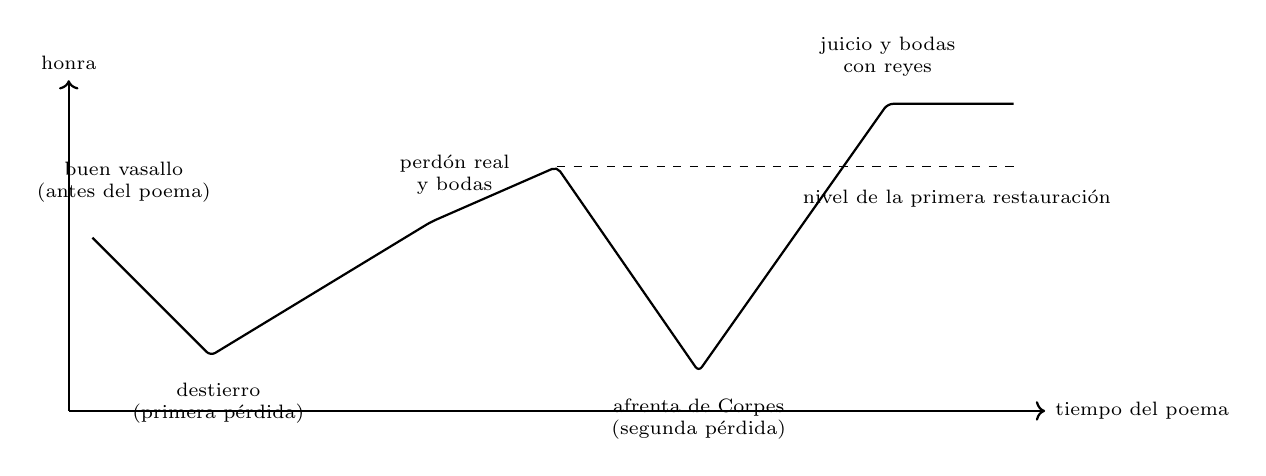
\begin{tikzpicture}
\tikzset{every node/.append style={align=center}}

\draw[->, thick] (0,0) -- (12.4,0) node[right, font=\scriptsize] {tiempo del poema};
\draw[->, thick] (0,0) -- (0,4.2) node[above, font=\scriptsize] {honra};
\draw[thick, rounded corners=2pt] (0.3,2.2) -- (1.8,0.7) -- (4.6,2.4) -- (6.2,3.1) -- (8.0,0.5) -- (10.4,3.9) -- (12.0,3.9);
\node[font=\scriptsize, align=center] at (0.7,2.9) {buen vasallo\\ (antes del poema)};
\node[font=\scriptsize, align=center] at (1.9,0.1) {destierro\\ (primera pérdida)};
\node[font=\scriptsize, align=center] at (4.9,3.0) {perdón real\\ y bodas};
\node[font=\scriptsize, align=center] at (8.0,-0.1) {afrenta de Corpes\\ (segunda pérdida)};
\node[font=\scriptsize, align=center] at (10.4,4.5) {juicio y bodas\\ con reyes};
\draw[dashed] (6.2,3.1) -- (12.0,3.1);
\node[font=\scriptsize, anchor=west] at (9.2,2.7) {nivel de la primera restauración};

\end{tikzpicture}
\end{document}
